% Options for packages loaded elsewhere
\PassOptionsToPackage{unicode}{hyperref}
\PassOptionsToPackage{hyphens}{url}
%
\documentclass[
]{book}
\usepackage{amsmath,amssymb}
\usepackage{lmodern}
\usepackage{iftex}
\ifPDFTeX
  \usepackage[T1]{fontenc}
  \usepackage[utf8]{inputenc}
  \usepackage{textcomp} % provide euro and other symbols
\else % if luatex or xetex
  \usepackage{unicode-math}
  \defaultfontfeatures{Scale=MatchLowercase}
  \defaultfontfeatures[\rmfamily]{Ligatures=TeX,Scale=1}
\fi
% Use upquote if available, for straight quotes in verbatim environments
\IfFileExists{upquote.sty}{\usepackage{upquote}}{}
\IfFileExists{microtype.sty}{% use microtype if available
  \usepackage[]{microtype}
  \UseMicrotypeSet[protrusion]{basicmath} % disable protrusion for tt fonts
}{}
\makeatletter
\@ifundefined{KOMAClassName}{% if non-KOMA class
  \IfFileExists{parskip.sty}{%
    \usepackage{parskip}
  }{% else
    \setlength{\parindent}{0pt}
    \setlength{\parskip}{6pt plus 2pt minus 1pt}}
}{% if KOMA class
  \KOMAoptions{parskip=half}}
\makeatother
\usepackage{xcolor}
\IfFileExists{xurl.sty}{\usepackage{xurl}}{} % add URL line breaks if available
\IfFileExists{bookmark.sty}{\usepackage{bookmark}}{\usepackage{hyperref}}
\hypersetup{
  pdftitle={Data Privacy Handbook},
  pdfauthor={Utrecht University},
  hidelinks,
  pdfcreator={LaTeX via pandoc}}
\urlstyle{same} % disable monospaced font for URLs
\usepackage{longtable,booktabs,array}
\usepackage{calc} % for calculating minipage widths
% Correct order of tables after \paragraph or \subparagraph
\usepackage{etoolbox}
\makeatletter
\patchcmd\longtable{\par}{\if@noskipsec\mbox{}\fi\par}{}{}
\makeatother
% Allow footnotes in longtable head/foot
\IfFileExists{footnotehyper.sty}{\usepackage{footnotehyper}}{\usepackage{footnote}}
\makesavenoteenv{longtable}
\usepackage{graphicx}
\makeatletter
\def\maxwidth{\ifdim\Gin@nat@width>\linewidth\linewidth\else\Gin@nat@width\fi}
\def\maxheight{\ifdim\Gin@nat@height>\textheight\textheight\else\Gin@nat@height\fi}
\makeatother
% Scale images if necessary, so that they will not overflow the page
% margins by default, and it is still possible to overwrite the defaults
% using explicit options in \includegraphics[width, height, ...]{}
\setkeys{Gin}{width=\maxwidth,height=\maxheight,keepaspectratio}
% Set default figure placement to htbp
\makeatletter
\def\fps@figure{htbp}
\makeatother
\setlength{\emergencystretch}{3em} % prevent overfull lines
\providecommand{\tightlist}{%
  \setlength{\itemsep}{0pt}\setlength{\parskip}{0pt}}
\setcounter{secnumdepth}{5}
\usepackage{booktabs}
\ifLuaTeX
  \usepackage{selnolig}  % disable illegal ligatures
\fi
\usepackage[]{natbib}
\bibliographystyle{apalike}

\title{Data Privacy Handbook}
\author{Utrecht University}
\date{2022-07-01}

\begin{document}
\maketitle

{
\setcounter{tocdepth}{1}
\tableofcontents
}
\hypertarget{welcome}{%
\chapter*{Welcome!}\label{welcome}}
\addcontentsline{toc}{chapter}{Welcome!}

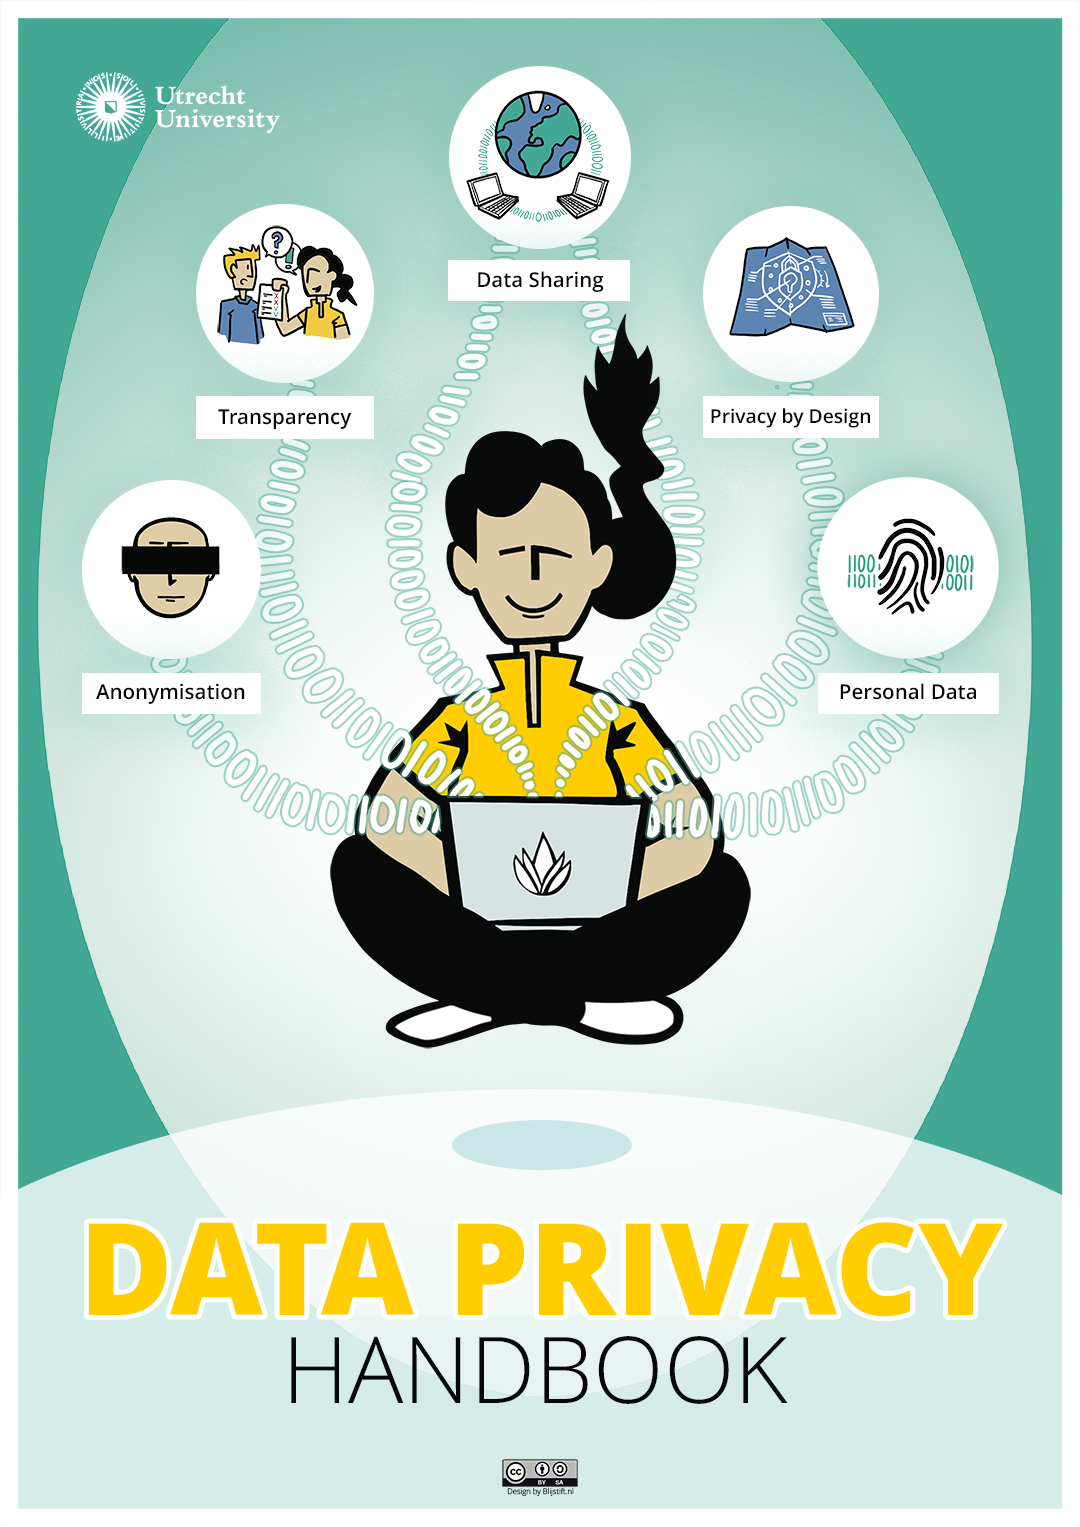
\includegraphics{img/cover-image-dph.png}

The Data Privacy Handbook is a guide on handling personal data in scientific
research, in line with European data protection and privacy regulations. It
consists of:

\begin{itemize}
\tightlist
\item
  A \textbf{knowledge base} which explains how the EU General Data Protection Regulation (GDPR, Dutch: Algemene Verordening Gegevensbescherming) applies to scientific research, including guidelines and good practices in carrying out GDPR-compliant scientific research;
\item
  An overview of privacy-enhancing \textbf{techniques \& tools} and practical guidance on their implementation;
\item
  \textbf{Use Cases} in the form of research projects with privacy-related issues, for which a reusable solution (e.g., tool, workflow) has been developed.
\end{itemize}

The Data Privacy Handbook synthesizes information across various sources and
presents it a \emph{practical} and \emph{actionable} format. This includes workflows,
tools, and practical translations of the GDPR , which could be used by researchers
and (data) support staff within Utrecht University and beyond.

This is an Utrecht University (UU) community-driven, open-source project.
You can visit our GitHub repository here.
We welcome feedback and contributions of any type, please read our
contributing guidelines
for more information.

The Data Privacy Handbook is an initiative of
Research Data Management Support
at the Utrecht University Library,
in collaboration with privacy and data experts at Utrecht University. It is part of a larger Data Privacy Project,
that aims to develop knowledge, tools, and experience on how researchers can and
should deal with personal data. This project is funded by the Utrecht University
Research IT Program and an NWO Digital Competence Center grant. You can read more
about the Data Privacy Project here.

\hypertarget{how-to-use-this-handbook}{%
\section{How to use this Handbook}\label{how-to-use-this-handbook}}

The Data Privacy Handbook aims to make knowledge and solutions on handling personal
data \emph{Findable, Accessible, Interoperable, and Reusable} (FAIR) and present them in
a practical and actionable format.

The Handbook need not be read like a textbook. You are invited to navigate to the
topic you need based on the table of contents, or use the guide below.

\hypertarget{what-are-you-looking-for}{%
\subsection{What are you looking for?}\label{what-are-you-looking-for}}

I want to\ldots:

Learn about the GDPR in the context of scientific research

Introduction to the GDPR

Definitions

Plan a GDPR-compliant research project

Assessing your design

Informing participants

Obtaining consent

Collaborating on personal data

Work safely with personal data

Storing personal data

Using GDPR-compliant tools and services

Reducing the sensitivity of personal data

Sharing personal data during research

Share personal data with others

Sharing data legally

Sharing personal data during research

Reducing the sensitivity of personal data

Using GDPR-compliant tools and services

Publishing personal data

Sharing personal data case by case

Learn from other projects

Publishing metadata only

Pseudonymising different types of data

Minimising personal data processing in a survey

Get help or information

Getting help at Utrecht University

Definitions

References

\hypertarget{license-and-citation}{%
\section{License and Citation}\label{license-and-citation}}

The Data Privacy Handbook is licensed under a Creative Commons Attribution 4.0 International License. You can view the license here.

\hypertarget{disclaimer}{%
\section{Disclaimer}\label{disclaimer}}

The content presented in the Data Privacy Handbook has been carefully curated by Research Data Management Support,
in collaboration with privacy officers and data experts of Utrecht University.

The Data Privacy Handbook is a `living' book that is continually being written, updated and reviewed. Its contents can
therefore change, or become outdated or redundant . Hence, the information presented is provided ``as is'', \textbf{without
guarantees of accuracy or completeness}.

As scientific research may differ depending on the discipline, topic, and context, measures needed or taken to ensure
GDPR-compliance will vary across research projects. The authors can therefore \textbf{not be held responsible, nor accountable}
for any negative consequences arising from interpretation and use of the content of the Data Privacy Handbook.

The Handbook is not endorsed by the Board of Utrecht University and does not constitute a mandatory directive.
For the most up-to-date and official/authoritative information, please refer to the
university website and
intranet, to which this Handbook is
a hands-on, practical supplement. Moreover, before implementing the guidance laid out in this Handbook, always seek
the advice of your privacy officer or RDM Support to confirm the suitability of any proposed solution to your project.

Throughout the Data Privacy Handbook, links to external webpages may be provided for additional information or assistance.
The authors of the Data Privacy Handbook are \textbf{not responsible for the content of any such linked webpages}, nor is the
content of external webpages necessarily endorsed by Utrecht University.

Utrecht University is committed to sharing knowledge in line with the principles of open science and therefore welcomes
readers from outside of the organization. However, the contents of the Data Privacy Handbook may not be in line with readers'
institutions' policies or views. For more authoritative information, these readers' should refer to resources from their own
institutions.

\hypertarget{contributions}{%
\section{Contributions}\label{contributions}}

The Data Privacy Handbook is a collaborative effort, made possible by a large number of contributors (also to be viewed
in our GitHub repository):

Neha Moopen, Dorien Huijser, Jacques Flores, Wies Cipido, Joris de Graaf, Judith de Haan, Saskia van den Hout, Frans Huigen, Artan Jacquet, Sanne Kleerebezem, Annemiek van der Kuil, Danny de Koning-van Nieuwamerongen, Frans de Liagre Böhl, Francisco Romero Pastrana, Najoua Ryane, Johanneke Siljee, Ron Scholten, Garrett Speed, Robert Steeman, Liliana Vargas Meleza, Martine de Vos, and others.

Would you like to contribute to this Handbook yourself? Please read our
Contributing Guidelines.

\hypertarget{faq}{%
\chapter{What are you looking for?}\label{faq}}

\hypertarget{part-knowledge-base}{%
\part{Knowledge Base}\label{part-knowledge-base}}

\hypertarget{gdpr}{%
\chapter*{The GDPR}\label{gdpr}}
\addcontentsline{toc}{chapter}{The GDPR}

\textbf{This chapter will present the most important definitions, principles and rights
of data subjects outlined in the GDPR and how it applies to your research. Most
of the practical advice that we provide in this Handbook will be rooted in and
builds on the concepts presented here.}

\hypertarget{chapter-summary}{%
\subsection{Chapter summary}\label{chapter-summary}}

The GDPR is a EU-wide regulation that controls the processing of personal data.
If you process personal data, you should:

\begin{itemize}
\tightlist
\item
  Make sure you have a legal basis to process the
  data. In research, this is often informed consent.
\item
  Be transparent and fair towards data subjects.
\item
  Be specific in which personal data you process and for what purposes. Limit
  the amount of data you process to what is necessary, and only store the data
  for that necessary amount of time.
\item
  Protect the confidentiality of the data by incorporating
  privacy by design into your project from the start.
\item
  Make sure your data subjects can exercise their
  data subjects' rights, and they know how to
  do so.
\end{itemize}

\hypertarget{what-is-the-gdpr}{%
\section{What is the GDPR?}\label{what-is-the-gdpr}}

The General Data Protection Regulation (GDPR, Dutch: \emph{Algemene Verordening
Gegevensbescherming} {[}AVG{]}) is an EU-wide regulation meant to protect the privacy
of individuals within a rapidly growing technological society. The GDPR facilitates
the free movement of personal data within the European Economic Area (EEA). Its
data processing principles are meant to ensure a fair balance between competing
interests -- for example, the right to conduct research vs.~the right to protect
personal data (Articles 13 and 8, from the Charter of Fundamental right of the EU).

\hypertarget{the-gdpr-in-a-nutshell}{%
\subsubsection{The GDPR in a nutshell}\label{the-gdpr-in-a-nutshell}}

All articles and recitals of the GDPR can be found online via \url{https://gdpr-info.eu/}.
The video below highlights some important aspects of the GDPR:

Click to read the English video transcript

The General Data Protection Regulation (GDPR) regulates what we can
and cannot do with personal data such as a person's name, sexual orientation,
home address and health. This also applies to personal data used in research
and education. The regulation consists of 88 pages. Fortunately, the basics
are easy to remember in 3 steps:

First, there must be a clear legal basis for processing personal data. This can
include consent, a legal obligation, or public interest.

Second, appropriate technical and organisational measures must be taken
while processing personal data to ensure maximum privacy.

Lastly, the persons whose data you have collected must always have the
option of inspecting, changing, or removing their personal data.

That is the GDPR in a nutshell.

\hypertarget{when-does-the-gdpr-apply}{%
\subsubsection{When does the GDPR apply?}\label{when-does-the-gdpr-apply}}

The GDPR has been applicable from May 2018 onward and applies when:

\begin{itemize}
\tightlist
\item
  you are processing personal data
  (material scope, art. 2).
\item
  the controller or processor of the data \emph{resides} in the EEA (territorial
  scope, art. 3).
  This is independent of whether the actual processing takes place in the EEA.
  In some cases, the GDPR also applies when the controller or processor is not
  established in the EEA, but is processing data from EU citizens.
\end{itemize}

\textbf{If you are collecting or using data that originated from individuals (or is
related to individuals), it is very likely that the GDPR applies to your project.}

\hypertarget{implementation}{%
\subsubsection{Implementation}\label{implementation}}

While the GDPR is a regulation for the entire EEA, each EEA country can additionally
implement further restrictions and guidelines in national implementation laws. The
Dutch implementation law is called ``Uitvoeringswet AVG (UAVG)''
(most recent version).
The UAVG determines, for example, that it is forbidden to process Citizen
Service Numbers (BSN), unless it is for purposes determined by a law or a
General Administrative Order (AMvB).

\hypertarget{definitions}{%
\section*{Definitions in the GDPR}\label{definitions}}
\addcontentsline{toc}{section}{Definitions in the GDPR}

Below, you will find a selection of important terms in the GDPR that you should
become familiar with when working with personal data (also included in the
Definitions). Click a term to see the definition.

Data subject

A living individual who can be identified directly or indirectly through
personal data. In a research setting, this would be the individual whose
personal data is being processed (see below for the definition of processing).

Personal data

Any information related to an identified or identifiable (living) natural
person. This can include identifiers (name, identification number, location
data, online identifier or a combination of identifiers) or factors specific
to the physical, physiological, genetic, mental, economic, cultural or social
identity of the person. Moreover, IP addresses, opinions, tweets, answers to
questionnaires, etc. may also be personal data, either by itself or through a
combination of one another.

Of note: as soon as you collect data related to a person that is identifiable,
you are processing personal data. Additionally, pseudonymised data is still
considered personal data. Read more in
Designing a GDPR-compliant research project.

Special categories of personal data

Any information pertaining to the data subject which reveals any of the below categories:

racial or ethnic origin

political opinions

religious or philosophical beliefs

trade union membership

genetic and biometric data when meant to uniquely identify someone

physical or mental health conditions

an individual's sex life or sexual orientation

The processing of these categories of data is prohibited, unless one of
the exceptions of Article 9
applies. For example, an exception applies when:

the data subject has provided explicit consent to process these data for
a specific purpose,

the data subject has made the data publicly available themselves,

processing is necessary for scientific archiving purposes.

Contact your privacy
officer if you wish to process special categories of personal data.

Processing

Any operation performed on personal data. This includes collection, storage,
organisation, alteration, analysis, transcription, sharing, publishing, deletion, etc.

Controller

The natural or legal entity that, alone or with others, determines or has an
influence on why and how personal data are processed. On an
organisational level, Utrecht University (UU) is the controller of personal
data collected by UU researchers and will be held responsible in case of GDPR
infringement. On a practical level, however, researchers (e.g., Principal
Investigators) often determine why and how data are processed, and are thus
fulfilling the role of controller themselves.

Processor

A natural or legal entity that processes personal data on behalf of the
controller. For example, when using a cloud transcription service, you often
need to send personal data (e.g., an audio recording) to the transcription
service for the purpose of your research, which is then fulfilling the role
of processor. When using such a third party, you must have a
data processing agreement in place.

Legal basis

Any processing of personal data should have a valid legal basis. Without it,
you are now allowed to process personal data at all. The GDPR provides 6 legal
bases which are explained further in this chapter.

Anonymous data

Any data where an individual is irreversibly de-identified, both directly
(e.g., through names and email addresses) and indirectly. The latter means
that you cannot identify someone:

by combining variables or datasets (e.g., a combination of date of birth,
gender and birthplace, or the combination of a dataset with its name-number key)

via inference, i.e., when you can deduce who the data are about (e.g.,
when profession is Dutch prime minister, it is clear who the data is about)

by singling out a single subject, such as through unique data points
e.g., someone who is 210 cm tall is relatively easy to identify)

Anonymous data are no longer personal data and thus not subject to GDPR
compliance. In practice, anonymous data may be difficult to attain and care
must be given that the data legitimately cannot be traced to an individual in
any way. The document
Opinion 05/2014 on Anonymisation Techniques
explains the criteria that must be met for data to be considered anonymous.

Pseudonymous data

Personal data that cannot lead to identification without additional
information, such as a key file linking pseudonyms to names. This additional
information should be kept separately and securely and makes for
de-identification that is reversible. Data are sometimes pseudonymised by
replacing direct identifiers (e.g., names) with a participant code (e.g.,
number). However, this may not always suffice, as sometimes it is still
possible to identify participants indirectly (e.g., through linkage, inference
or singling out). Importantly, pseudonymous data are still personal data and
therefore must be handled in accordance with the GDPR.

\hypertarget{gdpr-principles}{%
\section*{Principles in the GDPR}\label{gdpr-principles}}
\addcontentsline{toc}{section}{Principles in the GDPR}

\textbf{The GDPR has a number of principles at its core which dictate the (method of)
data processing. Every type of processing has to comply with these principles.
Understanding these principles is the first step to determining what type of
personal data can be collected and how they can processed.}

The GDPR principles are explained further below the image. The
next chapter will describe how to implement these
principles in your research. You can also always contact your
privacy officer for help.

\hypertarget{lawful-fair-and-transparent}{%
\subsubsection{1. Lawful, fair and transparent}\label{lawful-fair-and-transparent}}

When working with personal data, your processing should be:

Lawful
Make sure all your processing activities (e.g., data collection, storage,
analysis, sharing) have a legal basis. Ideally,
you should have determined your processing purposes (e.g., research questions)
in advance.

Fair

Consider the broad effects of your processing on the rights and dignity
of the data subject.

Give data subjects the possibility to exercise
their rights.

Avoid deception in the communication with data subjects: processing of
personal data should be in line with what they can expect.

The processing of personal data should not have a disproportionate
negative, unlawful, discriminating or misleading effect on data subjects.

Transparent
Be transparent in the communication to your data subjects about who is
processing the personal data (controllers, processors), which personal data is
processed, as well as why and for how long, and how data subjects can exercise
their rights (see the Legal documents chapter).
The information provided should be unambiguous, concise, easily accessible and
relevant and shared with data subjects before the start of your research.

\hypertarget{purpose-limitation}{%
\subsubsection{2. Purpose limitation}\label{purpose-limitation}}

You can only process (i.e., collect, analyse, store, share, etc.) personal data
for a specific purpose and only for as long as necessary to complete that purpose.
For example, if you specified that you would use the personal data only to answer
your specific research question, you cannot further share the personal data for
reuse purposes, as this would be an additional processing purpose. This means
that you need to \textbf{plan what you will do with the (collected) personal data in
advance and stick to that plan in order to be GDPR-compliant}.

In some cases (e.g., for cohort studies), it may not be possible to communicate
a specific research purpose in advance. In those cases, you may be able to use
``broad consent'' when possible. For more information on broad consent and which
conditions must be met in that case see the Legal
Documents chapter.

\hypertarget{further-processing}{%
\paragraph{Further processing}\label{further-processing}}

It may happen that you want to process personal data for \textbf{similar, but other
purposes} than previously specified, for example because you formulated a research
question that was not communicated with the data subjects. In these cases, the
GDPR provides some leeway: you can still process the personal data if the new
processing (e.g., the new research question) is \textbf{compatible} with the original
purpose. Your
privacy officer
can help you assess whether this is the case. Of note, \textbf{archiving} personal
research data after your research is finished is allowed in a research context
(art. 5.1(b)),
but provided that you still apply the GDPR's principles and put in place appropriate
safeguards (rec. 156).

\hypertarget{data-minimisation}{%
\subsubsection{3. Data minimisation}\label{data-minimisation}}

You can only process the personal data you need to for your predefined purpose(s),
and not more just because they may ``come in handy later''. This principle makes
sure that, for example, in the event of a data breach, the amount of data exposed
is kept to a minimum.

\hypertarget{accuracy}{%
\subsubsection{4. Accuracy}\label{accuracy}}

The accuracy of personal data is integral to data protection. Inaccurate data
can be a risk for data subjects, for example when they lead to a wrong treatment
in a medical trial. You therefore need to take every reasonable step to remove
or rectify data that is inaccurate or incomplete. Moreover, data subjects have
the right to request that inaccurate or
incomplete data be removed or rectified within 30 days.

\hypertarget{storage-limitation}{%
\subsubsection{5. Storage limitation}\label{storage-limitation}}

You can only store personal data for as long as is necessary to achieve your
(research) purpose. Afterwards, they need to be removed. If the personal data
are part of your research data (and not, for example, to simply contact data
subjects), you are allowed to store (archive) them for a longer period of time,
provided necessary safeguards are in place. This is an exemption that applies to
data storage for scientific archiving purposes. You need to inform the data
subjects on this storage duration beforehand.

N.B.: If identification of the data subject is no longer needed for your
(research) purposes, you do not need to keep storing the personal data just
to comply with the GDPR, even if it means your data subjects cannot exercise
their rights (art. 11).

\hypertarget{integrity-and-confidentiality}{%
\subsubsection{6. Integrity and confidentiality}\label{integrity-and-confidentiality}}

You have to process personal data securely and protect against unauthorised
processing or access, loss or damage. To this end, you should put in place
apropriate organisational and technical measures. The next chapter
will go into such measures in more depth.

\hypertarget{accountability}{%
\subsubsection{7. Accountability}\label{accountability}}

The controller is ultimately responsible for demonstrating GDPR-compliance. As a
researcher working with personal data, you are representing your institution
(e.g., Utrecht University) and you should therefore be able to demonstrate that
you process personal data in a compliant manner. Additionally, you should also
have some knowledge of data protection so that you can implement the right
measures into your research project.

\hypertarget{legal-basis}{%
\section*{When can I work with personal data?}\label{legal-basis}}
\addcontentsline{toc}{section}{When can I work with personal data?}

You can only process personal data if you have a \textbf{legal basis} to do so, which
should be registered, among other information, in the
processing register and
communicated to data subjects. There are 6 possible
legal bases which are outlined below. In research, the legal bases `informed
consent', `legitimate interests of the controller' and `public interest' are most
often used.

Please note that \textbf{for different purposes in your research project, a different
legal basis may apply}. For example, you may contact data subjects before they
start participating based on a legitimate interest and use informed consent for
collecting, storing, analysing and publishing the data.

\hypertarget{legal-bases-suitable-for-research}{%
\subsection{Legal bases suitable for research}\label{legal-bases-suitable-for-research}}

Informed consent

Informed consent is the most frequently used legal basis in research and
is often not only a legal (GDPR-consent), but also an ethical obligation
(e.g., METC informed consent). When using informed consent, you should
be able to demonstrate that the data subject was informed and has given
consent, and for which purpose(s) they gave their consent. In all cases,
consent has to be freely given, specific, informed and unambiguous. Please
refer to the Informed consent section
for guidance on applying informed consent in your research.

Legitimate interest of the controller

You can use this legal basis when processing personal data is necessary
for the legitimate interests of the controller (e.g., Utrecht University).
For example, this can be the case when you need to process contact
information to approach data subjects to participate, and you can only
obtain their consent after contacting them. Since contacting data subjects
is a prerequisite to perform your research, it can be in the university's
legitimate (research) interest to process their contact information. To
evaluate whether you can use legitimate interest as a legal basis, you
always need to weigh the interests of the controller (e.g., Utrecht
University) and the data subjects in a
Legitimate interest assessment.
Please contact your privacy officer to assess whether you can use this
legal basis in your research.

Public interest

This legal basis can only be used if it can be demonstrated that there
is an urgent social necessity for the processing of personal data. This
means that there must be an explicit increase in knowledge in the
interest of society. There is currently some disagreement as to when this
legal basis can be applied in research. Therefore, please contact your
privacy officer
to assess whether you can use this legal basis in your research.

\hypertarget{legal-bases-not-suitable-for-reseach}{%
\subsection{Legal bases not suitable for reseach}\label{legal-bases-not-suitable-for-reseach}}

Processing is necessary because of a legal obligation of the controller

This basis is not suitable for research. As an example, Utrecht
University has to share tax data with the Dutch tax administration in
order to comply with tax legislation.

Processing is necessary for the performance of a contract

This basis is not suitable for research. As an example, Utrecht
University has contracts with its employees, which require it to manage
the employees' financial data.

Processing is necessary to protect a person's vital interests

This basis is generally not suitable for research. If processing
someone's personal data is crucial to their health or even life, that
processing is allowed under the GDPR.

\hypertarget{data-subject-rights}{%
\section*{Data Subject's Rights}\label{data-subject-rights}}
\addcontentsline{toc}{section}{Data Subject's Rights}

The GDPR provides data subjects with several rights that gives them a relatively
high degree of control over their own personal data. Below, we list these rights
and how you can apply them in your research:

Right to be informed

Data subjects need to be clearly informed about what you are doing with their
personal data (a.o. art. 12).
This usually happens via a \emph{privacy notice} or \emph{information letter}. This right
does not apply if your research will be seriously harmed by meeting it and if
you haven't obtained the personal data directly from the data subjects themselves.

Right of access

Data subjects have the right to access a copy of the personal data you have
on them and to know what you are doing with that personal data and why
(art. 15).

Right to rectification

Data subjects have the right to correct and complement the personal data
that you have of them
art. 16).

Right to erasure/Right to be forgotten

Data subjects have the right to have their personal data removed (i.e.,
equivalent to the right to withdraw consent,
art. 17).
This right does \textbf{not} need to be granted if:

the personal data are published and need to be archived for validation
purposes.

it would seriously obstruct the research purpose(s).

it would hinder complying with a legal obligation or carrying out a task
in the public interest.

If the personal data have already been made public or shared, you need to
take reasonable measures to inform other users of the data of the erasure
request. A privacy officer can help you with this.

Right to restriction of processing:

Data subjects have the right to have you process less of their personal data
(art. 18),
for example if their personal data are inaccurate or your processing of it
is unlawful or no longer needed.

Right to data portability:

Data subjects have the right to have their personal data transferred to
another party (art. 20).

Right to object:

Data subjects have the right to object to what you are doing with their
personal data. This right applies when the processing is based on legitimate
or public interest (art. 21).
In case of objection, you have to stop your processing activities, unless
you can demonstrate grounds for overriding the data subject's rights.

\hypertarget{how-can-data-subjects-exercise-their-rights}{%
\subsubsection{How can data subjects exercise their rights?}\label{how-can-data-subjects-exercise-their-rights}}

Data subjects need to be \textbf{informed} about their rights and who to contact in
order to exercise them, including when you use a legal basis other than informed
consent. In research, this is usually done via a
privacy notice or information letter, which states
a contact person responsible for handling questions and requests.

Incoming requests need to be \textbf{coordinated with a privacy officer}, so that
they can be picked up in accordance with the GDPR. Additionally, at Utrecht
University, data subjects can always contact
\href{mailto:privacy@uu.nl}{\nolinkurl{privacy@uu.nl}} (the Data Protection Officer) for
requests or complaints.

\hypertarget{what-to-do-when-receiving-a-request-concerning-data-subjects-rights}{%
\subsubsection{What to do when receiving a request concerning data subjects' rights?}\label{what-to-do-when-receiving-a-request-concerning-data-subjects-rights}}

You have to provide a substantive response to the data subject \textbf{within 30 days},
in the same way as you received the request. Depending on the complexity and
number of requests, the response period may be extended by 2 months. In that
case, you must inform the data subject about this extension (including the
motivation) within one month. If needed, you can (and sometimes should) ask for
additional information to confirm the data subject's identity.

For granting requests about data subjects' rights, there should be a procedure
in place, in which you should at least consider:

\begin{itemize}
\tightlist
\item
  how you are going to retrieve the data (e.g., using a name-number key)
\item
  who is responsible for granting the request and informing the data subject
  about it (e.g., a data manager)
\item
  how the request is going to be granted, for example how they will be sent
  securely (access, portability), removed (forgotten, object, restriction) or
  corrected (rectification)
\end{itemize}

For larger projects, it may be wise to put a Standard Operating Procedure (SOP)
in place.

\hypertarget{what-if-the-data-have-already-been-anonymised}{%
\subsubsection{What if the data have already been anonymised?}\label{what-if-the-data-have-already-been-anonymised}}

The principles of data minimisation and storage limitation are considered more
important than keeping personal data just for the sake of identification
(art. 11).
Therefore, when receiving a request about anonymised data, you can make it clear
that you cannot retrieve the data subject's personal data, because they have
been anonymised. In this case, \textbf{the data subject cannot exercise their rights
anymore}. If you can still retrieve the data subject's personal data in some
way (i.e., when data are pseudonymised), you are \textbf{obliged to retrieve them}.
In order to do so, you can (and sometimes should) ask for additional information
that can confirm the data subject's identity.

\hypertarget{personal-data}{%
\chapter{What is personal data?}\label{personal-data}}

\hypertarget{privacy-by-design}{%
\chapter{Designing your project}\label{privacy-by-design}}

\hypertarget{risk-assessment}{%
\chapter{Privacy \& Security Assessment}\label{risk-assessment}}

\hypertarget{legal-documents}{%
\chapter*{Legal Documents \& Agreements}\label{legal-documents}}
\addcontentsline{toc}{chapter}{Legal Documents \& Agreements}

\hypertarget{privacy-notices}{%
\section*{Privacy Notices}\label{privacy-notices}}
\addcontentsline{toc}{section}{Privacy Notices}

\hypertarget{informed-consent-forms}{%
\section*{Informed Consent Forms}\label{informed-consent-forms}}
\addcontentsline{toc}{section}{Informed Consent Forms}

\hypertarget{legitimate-interest-assessment}{%
\section*{Legitimate Interest Assessment}\label{legitimate-interest-assessment}}
\addcontentsline{toc}{section}{Legitimate Interest Assessment}

\hypertarget{data-use-agreementconfidentiality-agreementnon-disclosure-agreement}{%
\section{Data Use Agreement/Confidentiality Agreement/Non-Disclosure Agreement}\label{data-use-agreementconfidentiality-agreementnon-disclosure-agreement}}

\hypertarget{data-transfer-agreement}{%
\section*{Data Transfer Agreement}\label{data-transfer-agreement}}
\addcontentsline{toc}{section}{Data Transfer Agreement}

\hypertarget{consortium-agreement-andor-joint-controller-agreement}{%
\section{Consortium Agreement and/or Joint Controller Agreement}\label{consortium-agreement-andor-joint-controller-agreement}}

\hypertarget{data-processing-agreement}{%
\section*{Data Processing Agreement}\label{data-processing-agreement}}
\addcontentsline{toc}{section}{Data Processing Agreement}

\hypertarget{part-techniques-tools}{%
\part{Techniques \& Tools}\label{part-techniques-tools}}

\hypertarget{privacy-enchancing-techniques}{%
\chapter{Privacy-Enhancing Techniques in Working With Personal Data}\label{privacy-enchancing-techniques}}

\hypertarget{anonymization}{%
\section{Anonymization}\label{anonymization}}

\hypertarget{pseudonymization}{%
\section{Pseudonymization}\label{pseudonymization}}

\hypertarget{encryption}{%
\section{Encryption}\label{encryption}}

\hypertarget{synthetic-data}{%
\section{Synthetic Data}\label{synthetic-data}}

\hypertarget{federated-analysis}{%
\section{Federated Analysis}\label{federated-analysis}}

\hypertarget{tools-and-services}{%
\chapter{Tools \& Services}\label{tools-and-services}}

\hypertarget{tools.uu.nl}{%
\section{tools.uu.nl}\label{tools.uu.nl}}

\hypertarget{survey-tools}{%
\section{Survey Tools}\label{survey-tools}}

\hypertarget{transcription-tools}{%
\section{Transcription Tools}\label{transcription-tools}}

\hypertarget{part-storage-sharing-publication}{%
\part{Storage, Sharing, Publication}\label{part-storage-sharing-publication}}

\hypertarget{data-storage}{%
\chapter{Storing personal data}\label{data-storage}}

In research, storage of personal data is one of the most common processing
activities. Assuming you have a legal basis to store personal data, you
then need to:

\begin{itemize}
\tightlist
\item
  Choose a storage medium that is GDPR-compliant and that provides a sufficient
  level of data protection;
\item
  Take into account procedural and legal aspects, e.g., how will you handle the
  data once they are stored, and for how long will you store the data?
\end{itemize}

These aspects of storing personal data are discussed in this chapter.

\hypertarget{chapter-summary-1}{%
\subsection{Chapter summary}\label{chapter-summary-1}}

\textbf{Where should I store personal data?}

Use a medium that has been approved by your institution. If you work at Utrecht
University, and your preferred storage medium is not included in the
Storage Finder,
then please contact
RDM Support
or your privacy officer
to find an alternative solution.

\textbf{How to store personal data?}

\begin{itemize}
\tightlist
\item
  Apply organisational and technical safeguards,
  e.g., restrict access, encrypt data, pseudonymise data, specify responsibilities, etc.
\item
  Store (personal) data preferably in a structured, commonly used, machine-readable
  and interoperable format: others should be able to open, understand and work
  with your data.
\end{itemize}

\textbf{For how long should I store personal data?}

\begin{itemize}
\tightlist
\item
  Delete or fully anonymise personal data when they are no longer necessary,
  and preferably determine when you will do this in advance.
\item
  In research, you can archive personal data that are necessary for validation
  purposes for a longer period of time, e.g., 10 years or longer.
\end{itemize}

\hypertarget{data-storage-where}{%
\section{Where should I store personal data?}\label{data-storage-where}}

\hypertarget{storage-media-at-uu}{%
\subsection{Storage media at UU}\label{storage-media-at-uu}}

If you work at Utrecht University (UU), you can find a suitable storage medium for
digital research data via the Storage Finder
(also embedded below). For personal data, select Basic, Sensitive or Critical
(depending on the sensitivity of your data) under question 4 about Confidentiality.

Most storage media in this overview are suitable for storing personal data, either
because they are controlled by UU (e.g., U- and O-drive, Beta File System) or
because UU has a Data Processing Agreement in place with the storage supplier
(e.g., Microsoft Office 365, Yoda, SURFdrive).

Please note:

\begin{itemize}
\tightlist
\item
  \textbf{Do not store personal research data on public cloud services}, e.g., Google
  Drive, Dropbox, OneDrive, Box, Mega, iDrive, iCloud, NextCloud, etc. These services
  are not (always) GDPR-compliant and/or may not offer sufficient data security.
  Moreover, UU does not have any formal agreements with these services, enabling
  them to use the data stored on their platforms for their own purposes.
\item
  Only store data on personal or portable devices in an encrypted form.
\item
  When storing physical personal data (e.g., paper questionnaires, informed
  consent forms), you should lock the storage area (e.g., room, cabinet, drawer)
  and not leave unsecured copies of the data lying around (e.g., on a desk or printer).\\
\item
  Is your preferred storage medium not included in the storage finder? Contact
  RDM Support,
  your data steward, or your
  privacy officer
  to find an alternative solution.
\end{itemize}

\textbf{If you work at UU, please find a suitable storage medium below:}

\hypertarget{data-storage-requirements}{%
\section{Requirements for a suitable storage medium}\label{data-storage-requirements}}

\textbf{Whether a storage medium is suitable for storing personal data depends on 1) who
is controlling the personal data, and 2) the security measures of the storage
medium. If you want to use a storage medium not recommended/offered by UU,
please consult with
RDM Support,
your data steward, or your
privacy officer.}

\hypertarget{who-is-storing-the-personal-data-arrange-an-agreement}{%
\subsection{1. Who is storing the personal data: arrange an agreement}\label{who-is-storing-the-personal-data-arrange-an-agreement}}

When you use an external storage provider, the data is not under the (full)
control of your employer. In this case, it is required to ensure GDPR compliance
of the storage provider using
(art. 46):

\begin{itemize}
\tightlist
\item
  A Data Processing Agreement -
  when storing personal data within the European Economic Area (EEA) or a
  country with an
  adequate level of data protection.
\item
  Standard
  contractual clauses (SCCs) - when storing personal data with a
  supplier outside of the EEA. These make sure the storage medium will use
  sufficient measures to protect the personal data and enable data subjects to
  exercise their rights.
\item
  Explicit consent of data subjects who have been informed on the risks
  involved - in the absence of an agreement. Please contact your
  privacy officer
  if you are considering this option.
\end{itemize}

You can assume agreements are in place for the storage media recommended by UU.
If there is no agreement in place between UU and the storage provider, using
this storage provider is \textbf{not allowed}, even if they are located within the EEA,
have an adequate level of data protection, or have high security standards. The
only exception is when data are always end-to-end encrypted, because then the
storage provider cannot learn anything from the data.

\hypertarget{security-of-the-storage-medium}{%
\subsection{2. Security of the storage medium}\label{security-of-the-storage-medium}}

The storage medium should employ good security practices, such as regular back-ups
in distinct geographical areas (preferably in replication rather than on tape),
regular integrity checks, encryption at rest, multi-factor authentication, etc.
Most of these aspects will likely be covered in the agreement. Information
security can help determine all necessary security requirements.

\hypertarget{data-storage-how}{%
\section{How should I store personal data?}\label{data-storage-how}}

\textbf{Once you have chosen a suitable storage medium, you should act in accordance
with the nature of your data as well}, for example through:

\begin{itemize}
\tightlist
\item
  Controlling access: make sure that only the necessary people have the right
  kind of access (e.g.~read/write) to the personal data, and remove their access
  when they do not longer need it (e.g.~when someone leaves the research project).\\
\item
  Specifying responsibilities, e.g.~who is responsible for guarding access to the
  data on both the short and the long term? Make people aware of the confidential
  nature of the data. Tell them what to do in case of a
  data breach.
\item
  Procedural arrangements, e.g.~capture access conditions in
  agreements like the consortium agreement,
  data processing agreement or non-disclosure agreement.
\item
  Applying other safeguards where appropriate. For example, you can separate
  different types of personal data, encrypt, anonymise or pseudonymise the data,
  etc. (see chapter Privacy-enhancing techniques).
\end{itemize}

See Designing a GDPR-compliant research project for more tips.

Personal data should be stored in a \textbf{``structured, commonly used, machine-readable
and interoperable format''} (rec. 68).
In practice, this means that you should consider whether your files are
structured and named in a logical way, use
sustainable file formats,
and provide understandable metadata so that others can interpret the data.
You can read more about this in the RDM guide
``Storing and preserving data''.

\hypertarget{data-storage-duration}{%
\section{For how long should I store personal data?}\label{data-storage-duration}}

\textbf{As per the GDPR, anyone processing personal data can only store those for as
long as is necessary for prespecified purposes
(art. 5(e)).
Afterwards, the personal data have to either be fully anonymised or deleted.
However, there is an exemption for research data, as described below.}

In practice, in research we often see a division in two types of retention periods:

\begin{itemize}
\tightlist
\item
  If the personal data underpin a scientific publication, it is usually necessary
  to archive some personal data for \textbf{integrity and validation purposes}
  (art. 5(e)).
  At UU, any research data necessary for validation should be archived for at least
  10 years (UU research data policy).
  If this includes personal data, they too should be archived. Importantly, this
  still means that you need to \textbf{protect} the personal data, and \textbf{limit} the personal
  data stored to the amount necessary for validation
  (art. 89)!
  This also implies that you should keep the documentation about the legal basis
  used (e.g., consent forms) during that time, so that you can demonstrate GDPR
  compliance.
\item
  Personal data that were used for purposes other than answering your
  research question (e.g.~contact information) should have their own retention
  policy: they should be removed or anonymised after the retention period
  (e.g.~the research project) has ended.
\end{itemize}

For all types of data in your project (incl.~to be archived research data), we
recommend to formulate which data you will retain and for how long (for example
in your Data Management Plan), and communicate the (possibly different)
retention period(s) to data subjects. If you want to change the storage term you
initially set and communicated for your personal data, please contact your
privacy officer.

\hypertarget{deleting-personal-data}{%
\subsection{Deleting personal data}\label{deleting-personal-data}}

If you do not need personal data anymore, you must delete it. Data deletion
should be done in a reliable manner, for example to ensure that there are no
visible or hidden copies being left behind on any device. The
Storage Finder
will soon include information on how to do this for each UU-approved storage medium.
Additionally, you can read more on how to safely delete data in the RDM guide
``Storing
and preserving data''.

\hypertarget{data-sharing}{%
\chapter{Data Sharing}\label{data-sharing}}

\hypertarget{can-i-share-personal-data}{%
\section{Can I Share Personal Data?}\label{can-i-share-personal-data}}

\hypertarget{third-country-transfers}{%
\section{Third Country Transfers}\label{third-country-transfers}}

\hypertarget{data-access-protocols}{%
\section{Data Access Protocols}\label{data-access-protocols}}

\hypertarget{data-pointsvirtual-research-environments}{%
\section{Data Points/Virtual Research Environments}\label{data-pointsvirtual-research-environments}}

\hypertarget{data-publishing}{%
\chapter{Data Publishing}\label{data-publishing}}

\hypertarget{publishing-personal-data}{%
\section{Publishing Personal Data}\label{publishing-personal-data}}

\hypertarget{data-vs.-metadata}{%
\section{Data vs.~Metadata}\label{data-vs.-metadata}}

\hypertarget{repositories}{%
\section{Repositories}\label{repositories}}

\hypertarget{licenses}{%
\section{Licenses}\label{licenses}}

\hypertarget{part-use-cases}{%
\chapter{(PART) Use Cases}\label{part-use-cases}}

\hypertarget{open-science-questionnaire}{%
\chapter{Publishing metadata}\label{open-science-questionnaire}}

\hypertarget{youth-pseudonymisation}{%
\chapter{Data pseudonymisation}\label{youth-pseudonymisation}}

\hypertarget{pet-survey}{%
\chapter{Data minimisation in a survey}\label{pet-survey}}

The glossary consists of frequently used jargon concerning the GDPR and research data.

\hypertarget{a}{%
\subsubsection{A}\label{a}}

Anonymous data

Any data where an individual is irreversibly de-identified, both directly (e.g., through names and email addresses) and indirectly. The latter means that you cannot identify someone:

by combining variables or datasets (e.g., a combination of date of birth, gender and birthplace, or the combination of a dataset with its name-number key)

via inference, i.e., when you can deduce who the data are about (e.g., when profession is Dutch prime minister, it is clear who the data is about)

by singling out a single subject, such as through unique data points (e.g., someone who is 210 cm tall is relatively easy to identify)

Anonymous data are no longer personal data and thus not subject to GDPR compliance. In practice, anonymous data may be difficult
to attain and care must be given that the data legitimately cannot be traced to an individual in any way. The document
Opinion 05/2014 on Anonymisation Techniques
explains the criteria that must be met for data to be considered anonymous.

\hypertarget{c}{%
\subsubsection{C}\label{c}}

Controller

The natural or legal entity that, alone or with others, determines or has an influence on why and how
personal data are processed. On an organisational level, Utrecht University (UU) is the controller of personal data
collected by UU researchers and will be held responsible in case of GDPR infringement. On a practical level, however,
researchers (e.g., Principal Investigators) often determine why and how data are processed, and are thus fulfilling the
role of controller themselves.

\hypertarget{d}{%
\subsubsection{D}\label{d}}

Data subject

A living individual who can be identified directly or indirectly through personal data. In a research setting,
this would be the individual whose personal data is being processed (see below for the definition of processing).

\hypertarget{e}{%
\subsubsection{E}\label{e}}

European Economic Area (EEA)

The member states of the European Union and Iceland, Liechtenstein, and Norway. In total, the EEA now consists of
30 countries. The aim of the EEA is to enable the ``free movement of goods, people, services and capital'' between countries,
and this includes (personal) data (source:
Eurostat).

\hypertarget{l}{%
\subsubsection{L}\label{l}}

Legal basis

Any processing of personal data should have a valid legal basis. Without it, you are now allowed to process personal data at all.
The GDPR provides 6 legal bases: consent, legitimate interest, public interest, legal obligation, performance of a contract, vital
interest. Consent and public and legitimate interest are most often used in a research context.

\hypertarget{p}{%
\subsubsection{P}\label{p}}

Personal data

Any information related to an identified or identifiable (living) natural person, for example identifiers (name, identification number,
location data, online identifier or a combination of identifiers) or factors specific to the physical, physiological, genetic, mental,
economic, cultural or social identity of the person. Moreover, IP address, opinions, tweets, answers to questionnaires, etc. may also be
personal data, either by itself or through a combination of one another.

Of note: as soon as you process data related to a person that is identifiable, you are processing personal data. Additionally,
pseudonymised data is still considered personal data. Read more in Designing a GDPR-compliant research project.

Processing

Any operation performed on personal data, including collection, storage, organisation, alteration, analysis,
transcription, sharing, publishing, deletion, etc.

Processor

A natural or legal entity that processes personal data on behalf of the controller. For example, when using
a cloud transcription service, you often need to send personal data (e.g., an audio recording) to the transcription
service for the purpose of your research, which is then fulfilling the role of processor. When using such a third party,
you must have a data processing agreement in place.

Pseudonymous data

Personal data that cannot lead to identification without additional information,
such as a key file linking pseudonyms to names. This additional information should be kept separately and securely
and makes for deidentification that is reversible. Data are sometimes pseudonymised by replacing direct identifiers
(e.g., names) with a participant code (e.g., number). However, this may not always suffice, as sometimes it is still
possible to identify participants indirectly (e.g., through linkage, inference or singling out). Importantly, pseudonymous
data are still personal data and therefore must be handled in accordance with the GDPR.

\hypertarget{s}{%
\subsubsection{S}\label{s}}

Special categories of personal data

Any information pertaining to the data subject which reveals any of the below categories:

racial or ethnic origin

political opinions

religious or philosophical beliefs

trade union membership

genetic and biometric data when meant to uniquely identify someone

physical or mental health conditions

an individual's sex life or sexual orientation

The processing of these categories of data is
prohibited, unless one of the exceptions of
art. 9 applies.
For example, an exception applies when:

\begin{verbatim}
<ul>
    <li>the data subject has provided explicit consent to process these data for a specific purpose</li>
    <li>the data subject has made the data publicly available themselves </li>
    <li>processing is necessary for scientific archiving purposes</li>
  </ul><p>Contact 
  your <a href="https://intranet.uu.nl/en/knowledgebase/contact-privacy" target="_blank">privacy officer</a> 
  if you wish to process special categories of personal data.</p>
\end{verbatim}

  \bibliography{book.bib,packages.bib}

\end{document}
